% !TeX program = xelatex
\documentclass[a4paper,10pt]{article}

% ============================================================================
% ១. កញ្ចប់បណ្ណាល័យ និងការកំណត់ទំព័រ (Packages & Page Setup — តាមគំរូ ls_plan.tex)
% ============================================================================
\usepackage[a4paper, left=0.95cm, right=0.95cm, top=0.85cm, bottom=0.92cm, footskip=0.52cm]{geometry}
\usepackage{amsmath}
\usepackage{unicode-math}
\usepackage{fontspec}
\usepackage{longtable, array, multirow, colortbl}
\usepackage[table]{xcolor}
\usepackage{enumitem}
\usepackage{pifont}
\usepackage{fancyhdr}
\usepackage{tikz}
\usetikzlibrary{calc, arrows.meta, decorations.pathreplacing, patterns, positioning, babel}

\makeatletter
\let\@expl@@@mark@update@singlecol@structures@@\relax
\makeatother

% --- ប្រព័ន្ធស្វែងរកទីតាំងពុម្ពអក្សរស្វ័យប្រវត្តិ (Windows Local + Cloud Repo fonts/) ---
\providecommand{\NGSFindFonts}{%
  \IfFileExists{C:/Windows/Fonts/cambria.ttc}{%
    \def\NGSSysPath{C:/Windows/Fonts/}%
    \def\NGSUserPath{C:/Users/KIT/AppData/Local/Microsoft/Windows/Fonts/}%
  }{%
    \IfFileExists{./fonts/KhmerOSsiemreap.ttf}{\def\NGSSysPath{./fonts/}\def\NGSUserPath{./fonts/}}{%
    \IfFileExists{../fonts/KhmerOSsiemreap.ttf}{\def\NGSSysPath{../fonts/}\def\NGSUserPath{../fonts/}}{%
    \IfFileExists{../../fonts/KhmerOSsiemreap.ttf}{\def\NGSSysPath{../../fonts/}\def\NGSUserPath{../../fonts/}}{%
    \IfFileExists{../../../fonts/KhmerOSsiemreap.ttf}{\def\NGSSysPath{../../../fonts/}\def\NGSUserPath{../../../fonts/}}{%
    \IfFileExists{../../../../fonts/KhmerOSsiemreap.ttf}{\def\NGSSysPath{../../../../fonts/}\def\NGSUserPath{../../../../fonts/}}{%
    \IfFileExists{../../../../../fonts/KhmerOSsiemreap.ttf}{\def\NGSSysPath{../../../../../fonts/}\def\NGSUserPath{../../../../../fonts/}}{%
    \IfFileExists{../../../../../../fonts/KhmerOSsiemreap.ttf}{\def\NGSSysPath{../../../../../../fonts/}\def\NGSUserPath{../../../../../../fonts/}}{%
      \def\NGSSysPath{../../../../../../../fonts/}\def\NGSUserPath{../../../../../../../fonts/}%
    }}}}}}}%
  }%
}
\NGSFindFonts

% ============================================================================
% ២. កំណត់ពុម្ពអក្សរ (Fonts — តាមគំរូ ls_plan.tex)
% ============================================================================
\setmathfont[Path={\NGSSysPath}, FontIndex=1, Scale=1.02]{cambria.ttc}
\defaultfontfeatures{Ligatures=TeX}

\setmainfont[
  Path={\NGSUserPath},
  Extension=.ttf,
  Script=Khmer,
  BoldFont={KhmerOSsiemreap},
  BoldFeatures={FakeBold=1.8},
  ItalicFont={KhmerOSsiemreap},
  ItalicFeatures={FakeSlant=0.25},
  BoldItalicFont={KhmerOSsiemreap},
  BoldItalicFeatures={FakeBold=1.8, FakeSlant=0.25}
]{KhmerOSsiemreap}

\newfontfamily\muol[Path={\NGSUserPath}, Extension=.ttf, Script=Khmer]{KhmerOSmuollight}
\newfontfamily\Tacteing[Path={\NGSUserPath}, Extension=.TTF]{TACTENG}
\newfontfamily\TimesEn[Path={\NGSSysPath}, Extension=.ttf, BoldFont={timesbd}, ItalicFont={timesi}, BoldItalicFont={timesbi}]{times}
\newfontfamily\CalibriFont[Path={\NGSSysPath}, Extension=.ttf]{calibri}
\newfontfamily\CourierCirc[Path={\NGSSysPath}, Extension=.ttf]{cour}

\XeTeXlinebreaklocale "km"
\XeTeXlinebreakskip = 0pt plus 1pt minus 0.1pt

% ============================================================================
% ៣. ពណ៌ និងការតុបតែង (Colors & Styles)
% ============================================================================
\definecolor{stepbg}{HTML}{D9D9D9}
\definecolor{headgray}{HTML}{E6E6E6}
\definecolor{emphred}{HTML}{C00000}

\pagestyle{fancy}
\fancyhf{}
\renewcommand{\headrulewidth}{0pt}
\fancyfoot[R]{\CalibriFont\fontsize{9pt}{11pt}\selectfont\thepage}

\setlength{\parindent}{0pt}
\setlength{\parskip}{0pt}
\setlength{\tabcolsep}{4.5pt}
\setlength{\LTpre}{2pt}
\setlength{\LTpost}{2pt}

\newcolumntype{L}[1]{>{\raggedright\arraybackslash}p{#1}}
\newcolumntype{C}[1]{>{\centering\arraybackslash}p{#1}}

% ============================================================================
% ៤. ពាក្យបញ្ជាជំនួយ (Helper Macros)
% ============================================================================
\newcommand{\en}[1]{{\TimesEn #1}}
\newcommand{\enbf}[1]{{\TimesEn\bfseries #1}}
\newcommand{\khmflourish}{{\Tacteing\fontsize{15pt}{15pt}\selectfont 3}}
\newcommand{\wcirc}{{\CourierCirc\fontsize{9.5pt}{11pt}\selectfont o}}
\newcommand{\ditem}{{\fontsize{7.5pt}{10pt}\selectfont\ding{117}}\ }
\newcommand{\fiveE}[1]{\textcolor{emphred}{\CalibriFont\bfseries #1}}
\newcommand{\redsub}[1]{\textcolor{emphred}{#1}}
\newcommand{\timenote}[1]{\textcolor{emphred}{\textit{#1}}}
\newcommand{\stepheader}[1]{\multicolumn{3}{|c|}{\cellcolor{stepbg}\muol #1} \\ \hline}
\newcommand{\cfig}[1]{{\centering\vspace{3pt}#1\vspace{3pt}\par}}
\newcommand{\cnum}[1]{\mbox{\fontsize{10.5pt}{12pt}\selectfont\ding{\numexpr181+#1\relax}}}
\newcommand{\unit}[1]{\,\text{\en{#1}}}
\newcommand{\graybox}[1]{\colorbox{headgray}{\strut #1}}
\newcommand{\dbox}{\,\tikz[baseline=-0.3ex]\draw[black, line width=0.7pt] (0,0) rectangle (0.32cm,0.32cm);\,}

% ============================================================================
% ៥. រូបភាព TikZ ស-ខ្មៅ សម្រាប់បង្រៀនលើក្ដារខៀន និងសន្លឹកកិច្ចការ (B&W Diagrams)
% ============================================================================

% ១. E1 Engage: អន្ទាក់លេខខាងចុងចំពោះតួចែក 3 (23 vs 123)
\newcommand{\figEngageDIVTwoOne}{%
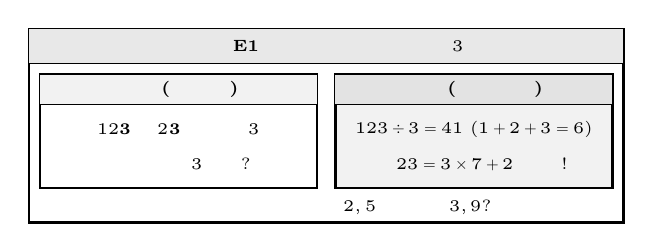
\begin{tikzpicture}[x=1cm, y=1cm, every node/.style={font=\fontsize{5.9pt}{7.8pt}\selectfont, text=black}]
  \draw[black, line width=0.9pt] (0,0) rectangle (7.55,2.46);
  \fill[gray!18] (0,2.02) rectangle (7.55,2.46);
  \draw[black, line width=0.6pt] (0,2.02) -- (7.55,2.02);
  \node at (3.775,2.24) {\textbf{បេសកកម្ម \en{E1}៖ អន្ទាក់ការមើលតែខ្ទង់រាយលើភាពចែកដាច់នឹង $3$}};

  % Student A
  \draw[black, line width=0.8pt] (0.14,0.44) rectangle (3.66,1.88);
  \fill[gray!10] (0.14,1.50) rectangle (3.66,1.88);
  \draw[black, line width=0.5pt] (0.14,1.50) -- (3.66,1.50);
  \node at (1.90,1.69) {\textbf{សិស្ស ក (មើលតែខ្ទង់រាយ)}};
  \node at (1.90,1.18) {$12\mathbf{3}$ និង $2\mathbf{3}$ បញ្ចប់ដោយលេខ $3$};
  \node at (1.90,0.74) {ដូច្នេះចែកដាច់នឹង $3$ ទាំងពីរ?};

  % Student B
  \draw[black, line width=0.95pt, fill=gray!10] (3.89,0.44) rectangle (7.41,1.88);
  \fill[gray!22] (3.89,1.50) rectangle (7.41,1.88);
  \draw[black, line width=0.55pt] (3.89,1.50) -- (7.41,1.50);
  \node at (5.65,1.69) {\textbf{សិស្ស ខ (ពិនិត្យផលបូកខ្ទង់)}};
  \node at (5.65,1.18) {$123\div 3 = 41$ ($1+2+3=6$)};
  \node at (5.65,0.74) {តែ $23 = 3\times 7 + 2$ មិនដាច់ទេ!};

  \node at (3.775,0.20) {\textbf{សំណួរ៖} ហេតុអ្វីមើលខ្ទង់រាយប្រើបានចំពោះ $2, 5$ តែមិនបានចំពោះ $3, 9$?};
\end{tikzpicture}}

% ២. E2 Explore: គ្រួសារទាំង ៣ នៃភាពចែកដាច់ (ទំ.១៥-១៧)
\newcommand{\figFamiliesDIVTwoOne}{%
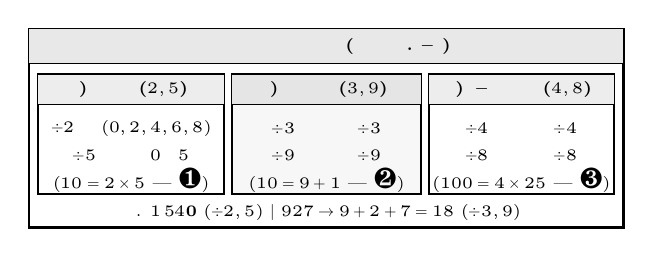
\begin{tikzpicture}[x=1cm, y=1cm, every node/.style={font=\fontsize{5.8pt}{7.7pt}\selectfont, text=black}]
  \draw[black, line width=0.9pt] (0,0) rectangle (7.55,2.52);
  \fill[gray!18] (0,2.08) rectangle (7.55,2.52);
  \draw[black, line width=0.6pt] (0,2.08) -- (7.55,2.08);
  \node at (3.775,2.30) {\textbf{គ្រួសារទាំង ៣ នៃលក្ខណៈចែកដាច់ (សៀវភៅគោល ទំ.១៥--១៧)}};

  % Family 1: Last digit (2, 5)
  \draw[black, line width=0.8pt] (0.12,0.42) rectangle (2.48,1.94);
  \fill[gray!14] (0.12,1.56) rectangle (2.48,1.94);
  \draw[black, line width=0.5pt] (0.12,1.56) -- (2.48,1.56);
  \node at (1.30,1.75) {\textbf{១) ខ្ទង់រាយ ($2, 5$)}};
  \node at (1.30,1.26) {$\div 2$៖ គូ ($0,2,4,6,8$)};
  \node at (1.30,0.92) {$\div 5$៖ ខ្ទង់រាយ $0$ ឬ $5$};
  \node at (1.30,0.60) {($10 = 2\times 5$ — \cnum{1})};

  % Family 2: Digit sum (3, 9)
  \draw[black, line width=0.8pt, fill=gray!6] (2.58,0.42) rectangle (4.98,1.94);
  \fill[gray!20] (2.58,1.56) rectangle (4.98,1.94);
  \draw[black, line width=0.5pt] (2.58,1.56) -- (4.98,1.56);
  \node at (3.78,1.75) {\textbf{២) ផលបូកខ្ទង់ ($3, 9$)}};
  \node at (3.78,1.26) {$\div 3$៖ ផលបូកខ្ទង់ $\div 3$};
  \node at (3.78,0.92) {$\div 9$៖ ផលបូកខ្ទង់ $\div 9$};
  \node at (3.78,0.60) {($10=9+1$ — \cnum{2})};

  % Family 3: Last 2 or 3 digits (4, 8)
  \draw[black, line width=0.8pt] (5.08,0.42) rectangle (7.43,1.94);
  \fill[gray!14] (5.08,1.56) rectangle (7.43,1.94);
  \draw[black, line width=0.5pt] (5.08,1.56) -- (7.43,1.56);
  \node at (6.255,1.75) {\textbf{៣) ២–៣ ខ្ទង់ចុង ($4, 8$)}};
  \node at (6.255,1.26) {$\div 4$៖ ២ ខ្ទង់ចុង $\div 4$};
  \node at (6.255,0.92) {$\div 8$៖ ៣ ខ្ទង់ចុង $\div 8$};
  \node at (6.255,0.60) {($100=4\times 25$ — \cnum{3})};

  \node at (3.775,0.19) {ឧ. $1\,54\mathbf{0}$ ($\div 2, 5$) $\mid$ $927 \to 9+2+7=18$ ($\div 3, 9$)};
\end{tikzpicture}}

% ៣. E4 Elaborate: លំហាត់គំរូ 11223[ ] ចែកដាច់នឹង 4 ផង និង 8 ផង (ទំ.១៧)
\newcommand{\figModelsDIVTwoOne}{%
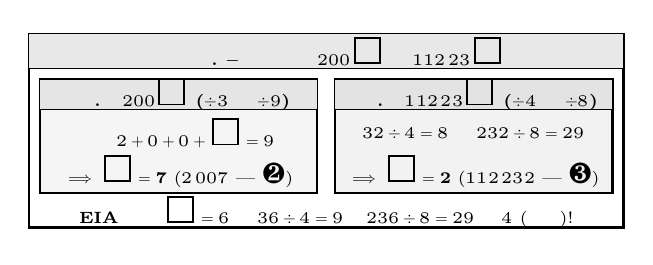
\begin{tikzpicture}[x=1cm, y=1cm, every node/.style={font=\fontsize{5.9pt}{7.8pt}\selectfont, text=black}]
  \draw[black, line width=0.9pt] (0,0) rectangle (7.55,2.46);
  \fill[gray!18] (0,2.02) rectangle (7.55,2.46);
  \draw[black, line width=0.6pt] (0,2.02) -- (7.55,2.02);
  \node at (3.775,2.24) {\textbf{លំហាត់គំរូ ទំ.១៦--១៧៖ បំពេញប្រអប់ $200\dbox$ និង $112\,23\dbox$}};

  % Left: 200[ ] div by 3 and 9
  \draw[black, line width=0.8pt, fill=gray!8] (0.14,0.44) rectangle (3.66,1.88);
  \fill[gray!20] (0.14,1.50) rectangle (3.66,1.88);
  \draw[black, line width=0.5pt] (0.14,1.50) -- (3.66,1.50);
  \node at (1.90,1.69) {\textbf{គំរូទំ.១៦៖ $200\dbox$ ($\div 3$ និង $\div 9$)}};
  \node at (1.90,1.20) {ផលបូក៖ $2 + 0 + 0 + \dbox = 9$};
  \node at (1.90,0.72) {$\implies \dbox = \mathbf{7}$ ($2\,007$ — \cnum{2})};

  % Right: 11223[ ] div by 4 and 8
  \draw[black, line width=0.85pt, fill=gray!10] (3.89,0.44) rectangle (7.41,1.88);
  \fill[gray!22] (3.89,1.50) rectangle (7.41,1.88);
  \draw[black, line width=0.5pt] (3.89,1.50) -- (7.41,1.50);
  \node at (5.65,1.69) {\textbf{គំរូទំ.១៧៖ $112\,23\dbox$ ($\div 4$ និង $\div 8$)}};
  \node at (5.65,1.20) {$32 \div 4 = 8$ និង $232 \div 8 = 29$};
  \node at (5.65,0.72) {$\implies \dbox = \mathbf{2}$ ($112\,232$ — \cnum{3})};

  \node at (3.775,0.20) {\textbf{\en{EIA}៖} បើដាក់ $\dbox = 6$ នោះ $36 \div 4 = 9$ តែ $236 \div 8 = 29$ សល់ $4$ (មិនដាច់)!};
\end{tikzpicture}}

% ៤. E5 Evaluate: សំណួរវិនិច្ឆ័យ A-D
\newcommand{\figExitDIVTwoOne}{%
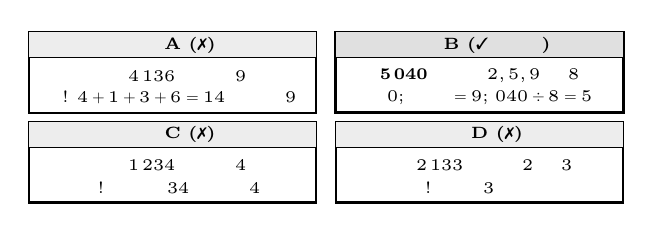
\begin{tikzpicture}[x=1cm, y=1cm, every node/.style={font=\fontsize{5.9pt}{7.6pt}\selectfont, text=black}]
  % Choice A
  \draw[black, line width=0.8pt] (0,1.14) rectangle (3.65,2.16);
  \fill[gray!14] (0,1.84) rectangle (3.65,2.16);
  \draw[black, line width=0.5pt] (0,1.84) -- (3.65,1.84);
  \node at (1.825,2.00) {\textbf{ជម្រើស \en{A} (\ding{55})}};
  \node at (1.825,1.61) {ចំនួន $4\,136$ ចែកដាច់នឹង $9$};
  \node at (1.825,1.33) {ខុស! $4+1+3+6=14$ មិនដាច់នឹង $9$};

  % Choice B (Correct)
  \draw[black, line width=1.05pt] (3.90,1.14) rectangle (7.55,2.16);
  \fill[gray!24] (3.90,1.84) rectangle (7.55,2.16);
  \draw[black, line width=0.6pt] (3.90,1.84) -- (7.55,1.84);
  \node at (5.725,2.00) {\textbf{ជម្រើស \en{B} (\ding{51} ត្រឹមត្រូវ)}};
  \node at (5.725,1.61) {$\mathbf{5\,040}$ ចែកដាច់នឹង $2, 5, 9$ និង $8$};
  \node at (5.725,1.33) {ចុង $0$; បូកខ្ទង់ $=9$; $040\div 8=5$};

  % Choice C
  \draw[black, line width=0.8pt] (0,0) rectangle (3.65,1.02);
  \fill[gray!14] (0,0.70) rectangle (3.65,1.02);
  \draw[black, line width=0.5pt] (0,0.70) -- (3.65,0.70);
  \node at (1.825,0.86) {\textbf{ជម្រើស \en{C} (\ding{55})}};
  \node at (1.825,0.47) {ចំនួន $1\,234$ ចែកដាច់នឹង $4$};
  \node at (1.825,0.19) {ខុស! ២ ខ្ទង់ចុង $34$ មិនដាច់នឹង $4$};

  % Choice D
  \draw[black, line width=0.8pt] (3.90,0) rectangle (7.55,1.02);
  \fill[gray!14] (3.90,0.70) rectangle (7.55,1.02);
  \draw[black, line width=0.5pt] (3.90,0.70) -- (7.55,0.70);
  \node at (5.725,0.86) {\textbf{ជម្រើស \en{D} (\ding{55})}};
  \node at (5.725,0.47) {ចំនួន $2\,133$ ចែកដាច់នឹង $2$ និង $3$};
  \node at (5.725,0.19) {ខុស! ខ្ទង់រាយ $3$ ជាចំនួនសេស};
\end{tikzpicture}}

\begin{document}
\fontsize{10pt}{15.2pt}\selectfont

% ============================================================================
% ក្បាលរដ្ឋបាល (Administrative Header — តាមគំរូ ls_plan.tex)
% ============================================================================
{\centering
  {\muol\fontsize{11pt}{16pt}\selectfont ព្រះរាជាណាចក្រកម្ពុជា\par}
  {\muol\fontsize{11pt}{16pt}\selectfont ជាតិ សាសនា ព្រះមហាក្សត្រ\par}
  \vspace{-3pt}{\khmflourish\par}
}

\vspace{1pt}
{\muol\fontsize{10pt}{15.5pt}\selectfont
មន្ទីរអប់រំ យុវជន និងកីឡា ខេត្តកំពង់ធំ\par
ការិយាល័យអប់រំ យុវជន និងកីឡា ស្រុកកំពង់ស្វាយ\par
អនុវិទ្យាល័យព្រះក្រសាំង\par}

\vspace{2pt}
{\centering{\muol\fontsize{11.5pt}{17pt}\selectfont កិច្ចតែងការបង្រៀន\par}}
\vspace{2pt}

% --- ព័ត៌មានទូទៅ ---
{\hspace*{2.8cm}\renewcommand{\arraystretch}{1.08}
\begin{tabular}{@{}l@{\hspace{0.35cm}}p{2.9cm}@{\hspace{0.15cm}}c@{\hspace{0.25cm}}l@{}}
  - & មុខវិជ្ជា & : & គណិតវិទ្យា ថ្នាក់ទី៧ (ពីជគណិត) \\
  - & ចំណងជើងមេរៀន & : & មេរៀនទី២៖ តួចែកនិងពហុគុណ \\
  - & ចំណងជើងរង & : & ១.១ ភាពចែកដាច់នឹង $2, 5, 3, 9, 4$ និង $8$ (ទំ.១៥--១៧) \\
  - & រយៈពេល & : & ១ ម៉ោងសិក្សា (៥០ នាទី) \\
  - & បង្រៀនដោយ & : & ហុក ប៊ុនថែន \\
  - & កាលបរិច្ឆេទ & : & ថ្ងៃព្រហស្បតិ៍ ទី១២ ខែវិច្ឆិកា ឆ្នាំ២០២៦ \\
\end{tabular}\par}

\vspace{2pt}

% --- I. វត្ថុបំណង ---
{\muol\fontsize{10pt}{15.5pt}\selectfont \enbf{I.} វត្ថុបំណង\par}
\vspace{1pt}
{\renewcommand{\arraystretch}{1.10}
\begin{tabular}{@{}p{0.55cm}@{}p{2.35cm}@{\hspace{0.15cm}}c@{\hspace{0.25cm}}p{14.95cm}@{}}
  \hfill\wcirc\hspace{0.2cm} & វិជ្ជាសម្បទា & : & សិស្សប្រាប់បានពីលក្ខណៈចែកដាច់នៃចំនួនគត់នឹង $2, 5$ (មើលខ្ទង់រាយ) នឹង $3, 9$ (មើលផលបូកខ្ទង់) និងនឹង $4, 8$ (មើលពីរឬបីខ្ទង់ចុងក្រោយ) បានត្រឹមត្រូវតាមសៀវភៅគោលទំ.១៥--១៧ ។ \\
  \hfill\wcirc\hspace{0.2cm} & បំណិនសម្បទា & : & សិស្សកំណត់បានភាពចែកដាច់ដោយមិនបាច់ធ្វើប្រមាណវិធីចែកវែង និងបំពេញលេខក្នុងប្រអប់ដើម្បីឱ្យចំនួនចែកដាច់នឹង $2, 5, 3, 9, 4, 8$ លើសន្លឹកកិច្ចការបានត្រឹមត្រូវ ។ \\
  \hfill\wcirc\hspace{0.2cm} & ចរិយាសម្បទា & : & សិស្សមានភាពរហ័សរហួន ហ្មត់ចត់ក្នុងការពិនិត្យលក្ខខណ្ឌចែកដាច់រួមគ្នា និងសហការពិភាក្សាជាក្រុមដោយស្មារតីទទួលខុសត្រូវ ។ \\
\end{tabular}\par}

\vspace{2pt}

% --- II. សម្ភារៈឧបទេស ---
{\muol\fontsize{10pt}{15.5pt}\selectfont \enbf{II.} សម្ភារៈឧបទេស\par}
\vspace{1pt}
\hspace*{0.55cm}$\bullet$\ សៀវភៅសិក្សាគោលថ្នាក់ទី៧ (ទំ.១៥--១៧ និងទំ.២៤) ក្ដារខៀន ដីស/ហ្វឺត និង\textbf{សន្លឹកកិច្ចការសិស្សបំពេញចន្លោះ ស-ខ្មៅ} (កូដ \en{DIV21} ទំព័រ ១--២ សម្រាប់សិស្ស និងទំព័រ ៣ ប្លង់ក្ដារខៀន/ចម្លើយគ្រូ — គ្មានប្រើ \en{LCD})\par

\vspace{2pt}

% --- III. វិធីសាស្រ្តបង្រៀន ---
{\muol\fontsize{10pt}{15.5pt}\selectfont \enbf{III.} វិធីសាស្រ្តបង្រៀន\par}
\vspace{1pt}
{\renewcommand{\arraystretch}{1.08}
\begin{tabular}{@{}p{0.55cm}@{}p{2.35cm}@{\hspace{0.15cm}}c@{\hspace{0.25cm}}p{14.95cm}@{}}
  \hfill$\bullet$\hspace{0.2cm} & គោលវិធី & : & សិស្សមជ្ឈមណ្ឌល (សន្លឹកកិច្ចការបំពេញចន្លោះជាគោល + ការពិភាក្សាជាក្រុមតូច ៣ នាក់) \\
  \hfill$\bullet$\hspace{0.2cm} & យុទ្ធវិធីបង្រៀន & : & គំរូស្ថាបនានិយម \en{5Es} រួមបញ្ចូល \textbf{ការបែងចែកគ្រួសារតាមរចនាសម្ព័ន្ធគោលដប់ (\en{Place-Value Structural Grouping})} និង \textbf{ឧទាហរណ៍ផ្ទុយបំបែកអន្ទាក់ខ្ទង់រាយ (\en{Counter-Example Inquiry})} \\
\end{tabular}\par}

\vspace{2pt}

% --- IV. ដំណើរការបង្រៀន ---
{\muol\fontsize{10pt}{15.5pt}\selectfont \enbf{IV.} ដំណើរការបង្រៀន\par}

{\renewcommand{\arraystretch}{1.14}
\begin{longtable}{|L{5.50cm}|L{7.90cm}|L{4.80cm}|}
\hline
\multicolumn{1}{|c|}{\cellcolor{headgray}\muol សកម្មភាពគ្រូ} &
\multicolumn{1}{c|}{\cellcolor{headgray}\muol ខ្លឹមសារមេរៀន} &
\multicolumn{1}{c|}{\cellcolor{headgray}\muol សកម្មភាពសិស្ស} \\
\hline
\endfirsthead

\hline
\multicolumn{1}{|c|}{\cellcolor{headgray}\muol សកម្មភាពគ្រូ} &
\multicolumn{1}{c|}{\cellcolor{headgray}\muol ខ្លឹមសារមេរៀន} &
\multicolumn{1}{c|}{\cellcolor{headgray}\muol សកម្មភាពសិស្ស} \\
\hline
\endhead

% ==================== ជំហានទី១ (2min) ====================
\stepheader{ជំហានទី១ \enbf{(}រដ្ឋបាលថ្នាក់\enbf{)}}
$\bullet$ ពិនិត្យវត្តមាន អនាម័យ និងសណ្ដាប់ធ្នាប់ថ្នាក់រៀន \par
$\bullet$ រៀបចំក្រុមតូច ៣ នាក់តាមតុ និងចែក\textbf{សន្លឹកកិច្ចការសិស្ស (\en{DIV21} ទំព័រ ១–២)}
&
$\bullet$ រដ្ឋបាលថ្នាក់ អនាម័យ និងវិន័យសិក្សា \par
$\bullet$ ចែកសន្លឹកកិច្ចការម្នាក់ ១ សន្លឹក សម្រាប់បំពេញតាមដំណាក់កាល \en{E1--E5}
&
$\circ$ ប្រធានថ្នាក់រាយការណ៍វត្តមានសិស្ស \par
$\circ$ ទទួលសន្លឹកកិច្ចការ សរសេរឈ្មោះ និងអង្គុយតាមក្រុម ៣ នាក់ \\
\hline

% ==================== ជំហានទី២ (9min: កំណែ <=3m + រំលឹក 3m + E1 3m) ====================
\stepheader{ជំហានទី២ \enbf{(}កិច្ចការផ្ទះ \enbf{+} ទំនាក់ទំនងមេរៀនថ្មី\enbf{)}}
\ditem \textbf{កំណែកិច្ចការផ្ទះ ($\le\text{\enbf{3\,min}}$)} \par
$\bullet$ ហៅសិស្សផ្ទៀងផ្ទាត់ចម្លើយលំហាត់ទំ.១៤ លេខ ៨ និង លេខ ៩ លើក្ដារខៀនផ្នែកឆ្វេង
&
{\centering\redsub{កំណែកិច្ចការផ្ទះមេរៀនមុន (ទំ.១៤ លេខ ៨ និង លេខ ៩)}\par}
$\bullet$ \textbf{លេខ ៨៖} ក. $\mathbf{500}$ \quad ខ. $\mathbf{134}$ \quad គ. $\mathbf{37}$ \quad ឃ. $3\times 5^2 = \mathbf{75}$ \par
$\bullet$ \textbf{លេខ ៩៖} ក. $\mathbf{12}$ \quad ខ. $\mathbf{14}$ \quad គ. $\mathbf{140}$ \quad ឃ. $\mathbf{127 / 27}$
&
$\circ$ ផ្ទៀងចម្លើយលេខ ៨ និង លេខ ៩ រួចកែចូលសៀវភៅ \\[3pt]

\ditem \textbf{រំលឹកមេរៀនទាក់ទង (\enbf{3min})} \par
$\bullet$ សួរ៖ «តើចំនួនគត់គូបញ្ចប់ដោយលេខអ្វីខ្លះ? ហើយពេលចែកចំនួនគត់ $a$ នឹង $b$ ដាច់ តើសំណល់ស្មើប៉ុន្មាន?»
&
{\centering\redsub{រំលឹកចំនួនគត់គូ និងវិធីចែកដាច់}\par}
$\bullet$ ចំនួនគត់គូមានលេខខាងចុងជា $0, 2, 4, 6$ ឬ $8$ \par
$\bullet$ $a$ ចែកដាច់នឹង $b$ លុះត្រាតែសំណល់ស្មើ $0$ ($a = b\times q$)
&
$\circ$ ឆ្លើយ៖ «បញ្ចប់ដោយ $0,2,4,6,8$ ហើយចែកដាច់មានសំណល់ស្មើ $0$!» \\[3pt]

\fiveE{E1 - Engage (3min)} \timenote{(កុំទាន់ផ្ដល់ចម្លើយ)} \par
\ditem \textbf{បេសកកម្មអន្ទាក់ខ្ទង់រាយ (\en{E1})}
&
\redsub{បេសកកម្ម \en{E1}៖ មើលតែខ្ទង់រាយសម្រាប់តួចែក $3$ បានទេ?}
&
$\circ$ អានស្ថានភាពបញ្ហា \en{E1} \\[3pt]

$\bullet$ ឱ្យសិស្សពិភាក្សាជាគូប្រៀបធៀបការអះអាងរបស់សិស្ស ក និងសិស្ស ខ
&
$\bullet$ \textbf{សិស្ស ក៖} «$123$ និង $23$ បញ្ចប់ដោយ $3$ ចែកដាច់នឹង $3$ ទាំងពីរ!» \par
$\bullet$ \textbf{សិស្ស ខ៖} «$123$ ចែកដាច់ តែ $23$ មិនចែកដាច់នឹង $3$ ទេ!»
&
$\circ$ ពិភាក្សាជាគូ និងគូស \ding{51} ក្នុងប្រអប់ \en{E1} \\[3pt]

&
\cfig{\figEngageDIVTwoOne}
& \\
\hline

% ==================== ជំហានទី៣ (17min: E2 11m + E3 6m) ====================
\stepheader{ជំហានទី៣ \enbf{(}ខ្លឹមសារមេរៀនថ្មី\enbf{)}}
\fiveE{E2 - Explore (11min)} \par
$\bullet$ សរសេរចំណងជើង \textbf{មេរៀនទី២៖ តួចែកនិងពហុគុណ — ១.១ ភាពចែកដាច់} \par
\ditem \textbf{សកម្មភាព ១៖ គ្រួសារខ្ទង់រាយ $2$ និង $5$ (ទំ.១៥--១៦, \enbf{3.5min}, \en{E2-A})}
&
១. លក្ខណៈចែកដាច់នៃចំនួនគត់ $\to$ \textbf{១.១ ភាពចែកដាច់} \par
$\bullet$ \textbf{ក. ភាពចែកដាច់នឹង $2$ និង $5$ (ទំ.១៥)៖} $42, 56, 198, 210$ ចែកដាច់នឹង $2$ (គូ); $70, 95, 160, 525$ ចែកដាច់នឹង $5$ (ចុង $0$ ឬ $5$) \par
$\bullet$ \textbf{ប្រតិបត្តិទំ.១៦៖} $154\dbox$ ចែកដាច់នឹង $2$ ផង និង $5$ ផង $\implies \dbox = \mathbf{0}$
&
$\circ$ សង្កេតខ្ទង់រាយ និងបំពេញ $1\,540$ លើ \en{E2-A} \\[3pt]

\ditem \textbf{សកម្មភាព ២៖ គ្រួសារផលបូកខ្ទង់ $3$ និង $9$ (ទំ.១៦, \enbf{4min}, \en{E2-B})} \par
$\bullet$ ឱ្យសិស្សគណនាផលបូកលេខតាមខ្ទង់នៃ $195, 927, 1\,005$ និង $216, 828, 2\,106$ លើ \en{E2-B}
&
$\bullet$ \textbf{ខ. ភាពចែកដាច់នឹង $3$ និង $9$ (ទំ.១៦)៖} \par
\hspace*{0.2cm}១) $\div 3$៖ $195 \to 1+9+5=\mathbf{15}$; $927 \to \mathbf{18}$; $1\,005 \to \mathbf{6}$ (សុទ្ធតែ $\div 3$) \par
\hspace*{0.2cm}២) $\div 9$៖ $216 \to 2+1+6=\mathbf{9}$; $828 \to \mathbf{18}$; $2\,106 \to \mathbf{9}$ (សុទ្ធតែ $\div 9$)
&
$\circ$ បូកលេខតាមខ្ទង់ ឃើញផលបូកចែកដាច់នឹង $3$ និង $9$ \\[3pt]

\ditem \textbf{សកម្មភាព ៣៖ គ្រួសារពីរ/បីខ្ទង់ចុងក្រោយ $4$ និង $8$ (ទំ.១៧, \enbf{3.5min}, \en{E2-C})} \par
$\bullet$ ឱ្យសិស្សសង្កេតពីរខ្ទង់ចុង ($124, 832, 1\,000$) និងបីខ្ទង់ចុង ($3\,128, 5\,048, 7\,120$)
&
$\bullet$ \textbf{គ. ភាពចែកដាច់នឹង $4$ និង $8$ (ទំ.១៧)៖} \par
\hspace*{0.2cm}១) $\div 4$៖ មើល \textbf{២ ខ្ទង់ចុង} ($24, 32, 00$ ចែកដាច់នឹង $4$ ព្រោះ $100 = 4\times 25$) \par
\hspace*{0.2cm}២) $\div 8$៖ មើល \textbf{៣ ខ្ទង់ចុង} ($128, 048, 120$ ចែកដាច់នឹង $8$ ព្រោះ $1\,000 = 8\times 125$)
&
$\circ$ គូសបន្ទាត់ក្រោម ២ ខ្ទង់ និង ៣ ខ្ទង់ចុងក្រោយលើ \en{E2-C} \\[3pt]

&
\cfig{\figFamiliesDIVTwoOne}
& \\[3pt]

% --- E3 Explain (6min) ---
\fiveE{E3 - Explain (6min)} \par
$\bullet$ ដឹកនាំសិស្សសង្ខេបវិធាន «ជាទូទៅ» ទាំង ៣ ក្រុមលើក្ដារខៀនកណ្ដាល និង \en{E3}
&
$\bullet$ \textbf{សង្ខេបលក្ខណៈចែកដាច់ទាំង ៦ (ទំ.១៥--១៧)៖} \par
\hspace*{0.15cm}១) ចែកដាច់នឹង $\mathbf{2}$ (ចំនួនគត់គូ) $\mid$ នឹង $\mathbf{5}$ (លេខខាងចុង $0$ ឬ $5$) \par
\hspace*{0.15cm}២) ចែកដាច់នឹង $\mathbf{3}$ ឬ $\mathbf{9}$ កាលណា\graybox{ផលបូកលេខតាមខ្ទង់}ចែកដាច់នឹង $3$ ឬ $9$ \par
\hspace*{0.15cm}៣) ចែកដាច់នឹង $\mathbf{4}$ (\graybox{២ ខ្ទង់ចុង} $\div 4$) $\mid$ នឹង $\mathbf{8}$ (\graybox{៣ ខ្ទង់ចុង} $\div 8$)
&
$\circ$ បំពេញប្រអប់សង្ខេបក្បួនទាំង ៦ លើសន្លឹកកិច្ចការ \en{E3} \\[3pt]

$\bullet$ ភ្ជាប់\textbf{ធនាគារហេតុផល \cnum{1}} លើក្ដារខៀន និងសន្លឹកកិច្ចការ
&
\textbf{ធនាគារហេតុផល (\en{Warrant Bank})៖} \par
\cnum{1} \textbf{គ្រួសារខ្ទង់រាយ ($2, 5$)៖} គូ $\iff \div 2$; ចុង $0,5 \iff \div 5$; ចុង $0 \iff \div 2, 5$
&
$\circ$ ផ្ទៀងលេខកូដ \cnum{1} លើសន្លឹកកិច្ចការ \\[3pt]

$\bullet$ ភ្ជាប់\textbf{ធនាគារហេតុផល \cnum{2}} សម្រាប់តួចែក $3$ និង $9$
&
\cnum{2} \textbf{គ្រួសារផលបូកខ្ទង់ ($3, 9$)៖} បូកគ្រប់ខ្ទង់ចូលគ្នា ($\div 9 \implies \div 3$ ជានិច្ច)
&
$\circ$ ផ្ទៀងលេខកូដ \cnum{2} លើសន្លឹកកិច្ចការ \\[3pt]

$\bullet$ ភ្ជាប់\textbf{ធនាគារហេតុផល \cnum{3}} សម្រាប់តួចែក $4$ និង $8$
&
\cnum{3} \textbf{គ្រួសារ ២–៣ ខ្ទង់ចុង ($4, 8$)៖} ២ ខ្ទង់ចុង $\div 4$; ៣ ខ្ទង់ចុង $\div 8$ ($\div 8 \implies \div 4$)
&
$\circ$ ផ្ទៀងលេខកូដ \cnum{3} លើសន្លឹកកិច្ចការ \\[3pt]

$\bullet$ ភ្ជាប់\textbf{ធនាគារហេតុផល \cnum{4}} សម្រាប់ការដោះស្រាយលក្ខខណ្ឌរួមគ្នា
&
\cnum{4} \textbf{លក្ខខណ្ឌរួមគ្នា៖} បើត្រូវចែកដាច់នឹង $a$ ផង និង $b$ ផង ត្រូវផ្ទៀងលក្ខខណ្ឌទាំងពីរ!
&
$\circ$ ផ្ទៀងលេខកូដ \cnum{4} លើសន្លឹកកិច្ចការ \\
\hline

% ==================== ជំហានទី៤ (20min: E4 10m + E5 10m) ====================
\stepheader{ជំហានទី៤ \enbf{(}ពង្រីកចំណេះដឹង\enbf{)}}
\fiveE{E4 - Elaborate (10min)} \par
\ditem \textbf{លំហាត់គំរូទំ.១៥, ទំ.១៦ និងទំ.១៧ លើសន្លឹកកិច្ចការ \en{E4}} \par
$\bullet$ ឱ្យសិស្សដោះស្រាយលំហាត់គំរូទំ.១៥ ដោយមិនធ្វើវិធីចែក ($9\,018+1\,457$ និង $1\,995+1\,329$)
&
{\muol លំហាត់គំរូ} \textbf{(សៀវភៅគោល ទំ.១៥--១៧)៖} \par
$\bullet$ \textbf{គំរូទំ.១៥៖} ក. $1\,995+1\,329 = 3\,324$ ចែកដាច់នឹង $\mathbf{2}$ (ខ្ទង់រាយគូ $5+9=14$) \par
\hspace*{0.2cm}ខ. $9\,018+1\,457 = 10\,475$ ចែកដាច់នឹង $\mathbf{5}$ (ខ្ទង់រាយ $8+7=15$ ចុង $5$ — \cnum{1})
&
$\circ$ ពិនិត្យផលបូកខ្ទង់រាយ ឃើញ $3\,324$ ($\div 2$) និង $10\,475$ ($\div 5$) \\[3pt]

$\bullet$ ឱ្យសិស្សដោះស្រាយលំហាត់គំរូទំ.១៦ ($200\dbox$) និងគំរូ ១ ទំ.១៧ ($112\,23\dbox$)
&
$\bullet$ \textbf{គំរូទំ.១៦៖} $200\dbox$ ($\div 3$ និង $\div 9$) $\implies 2+0+0+7=9 \implies \dbox = \graybox{$7$}$ (\cnum{2}) \par
$\bullet$ \textbf{គំរូ ១ ទំ.១៧៖} $112\,23\dbox$ ($\div 4$ និង $\div 8$) $\implies 32\div 4=8,\ 232\div 8=29 \implies \dbox = \graybox{$2$}$
&
$\circ$ បំពេញប្រអប់ $\dbox = 7$ និង $\dbox = 2$ លើ \en{E4} \\[3pt]

$\bullet$ ឱ្យសិស្សដោះស្រាយគំរូ ២ ទំ.១៧ (ឆ្នាំចន្លោះ $1999$ ដល់ $2010$)
&
$\bullet$ \textbf{គំរូ ២ ទំ.១៧៖} ពីឆ្នាំ $1999$ ដល់ $2010$ ចែកដាច់នឹង $4$ ផង $8$ ផង៖ \graybox{$2000$ និង $2008$} (\cnum{3})
&
$\circ$ រកឃើញឆ្នាំ $2000$ និង $2008$ \\[3pt]

&
\cfig{\figModelsDIVTwoOne}
& \\[3pt]

$\bullet$ សួរសំណួរឆ្លុះបញ្ចាំង \textbf{\en{EIA Looking-Back} (1min)} លើ $112\,23\dbox$
&
\textbf{\en{EIA Looking-Back}៖} «បើសិស្សដាក់ $\dbox = 6$ ក្នុង $112\,236$ តើចែកដាច់នឹង $4$ ផង និង $8$ ផងដែរឬទេ?» ($\to$ ទេ! $36\div 4=9$ ត្រូវចំពោះ $4$ តែ $236\div 8 = 29$ សល់ $4$!)
&
$\circ$ ឆ្លុះបញ្ចាំងថាត្រូវពិនិត្យដល់ ៣ ខ្ទង់ចុងក្រោយសម្រាប់តួចែក $8$ \\[3pt]

% --- E5 Evaluate (10min) ---
\fiveE{E5 - Evaluate (10min)} \par
\ditem \textbf{ប្រតិបត្តិជាក្រុមតូច ៣ នាក់ (4min, សន្លឹកកិច្ចការ \en{E5})} \par
$\bullet$ ឱ្យក្រុមសិស្សដោះស្រាយប្រតិបត្តិទំ.១៦ ($7\dbox 8$) និងប្រតិបត្តិទំ.១៧ ($734\dbox 0$)
&
{\muol លំហាត់ប្រតិបត្តិ} \textbf{(សៀវភៅគោល ទំ.១៦ និង ទំ.១៧)៖} \par
$\bullet$ \textbf{ទំ.១៦ ($7\dbox 8$ ចែកដាច់នឹង $3$ និង $9$)៖} $7+\dbox+8 = 15+\dbox = 18 \implies \dbox = \graybox{$3$}$ ($738$) \par
$\bullet$ \textbf{ទំ.១៧ ($734\dbox 0$)៖} ក. $\div 4 \implies \dbox \in \graybox{$\{0, 2, 4, 6, 8\}$}$ $\mid$ ខ. $\div 8 \implies \dbox \in \graybox{$\{0, 4, 8\}$}$
&
$\circ$ សហការគណនាឃើញ $\dbox = 3$ និងរកគ្រប់ចម្លើយនៃ $734\dbox 0$ \\[3pt]

$\bullet$ ឱ្យក្រុមសិស្សផ្ទៀងផ្ទាត់និង\textbf{បិទបេសកកម្ម \en{E1} (2min)}
&
$\bullet$ \textbf{បិទបេសកកម្ម \en{E1}៖} \textbf{សិស្ស ខ} ត្រឹមត្រូវ! $23$ មានផលបូកខ្ទង់ $2+3=5$ មិនចែកដាច់នឹង $3$ ទេ (\cnum{2}) ។
&
$\circ$ បិទបេសកកម្ម \en{E1} ដោយបញ្ជាក់ហេតុផលផលបូកខ្ទង់ \\[3pt]

\ditem \textbf{សំណួរវិនិច្ឆ័យ \en{A--D} និងសំបុត្រចេញ (4min)} \par
$\bullet$ សរសេរជម្រើស \en{A--D} លើក្ដារខៀន
&
{\centering\textbf{សំណួរវិនិច្ឆ័យ \en{A--D}៖ តើប្រយោគមួយណាត្រឹមត្រូវ?}\par}
&
$\circ$ ពិនិត្យជម្រើសទាំង ៤ តាមក្បួនចែកដាច់ \\[3pt]

$\bullet$ ឱ្យសិស្សគូសរង្វង់លើសន្លឹកកិច្ចការ និងលើកម្រាមដៃ ១--៤ ព្រមគ្នា
&
$\bullet$ វិភាគជម្រើស \en{A} ($4\,136$), \en{B} ($\mathbf{5\,040}$), \en{C} ($1\,234$), \en{D} ($2\,133$) តាមលេខកូដ \cnum{1}--\cnum{4}
&
$\circ$ គូសរង្វង់លើសន្លឹកកិច្ចការ និងលើកម្រាមដៃ ២ (\textbf{ជម្រើស \en{B}}) \\[3pt]

&
\cfig{\figExitDIVTwoOne}
& \\[3pt]

$\bullet$ បញ្ជាក់ចម្លើយត្រូវ (\textbf{ជម្រើស \en{B}}) និងឱ្យបំពេញ\textbf{សំបុត្រចេញ ៦០ វិនាទី}
&
$\bullet$ \textbf{សំបុត្រចេញ៖} បំពេញលេខក្នុងប្រអប់ $4\,2\dbox 0$ ដើម្បីឱ្យចែកដាច់នឹង $9$ ($\implies \dbox = \mathbf{3}$) ។
&
$\circ$ បំពេញសំបុត្រចេញឃើញ $4\,230$ មុនបញ្ចប់ម៉ោង \\
\hline

% ==================== ជំហានទី៥ (<=2min) ====================
\stepheader{ជំហានទី៥ \enbf{(}កិច្ចការផ្ទះ \enbf{+} បណ្ដាំផ្ញើ\enbf{)}}
\timenote{ចំណាយពេលឱ្យតិចបំផុតកុំឱ្យលើស 2min} \par
$\bullet$ ណែនាំប្រអប់\textbf{កិច្ចការផ្ទះ}លើសន្លឹកកិច្ចការទំព័រ ២ (សៀវភៅគោល ទំ.២៤ លេខ ២ បូកពង្រឹង ១ ខ្ទង់)
&
{\centering{\muol កិច្ចការផ្ទះ} \textbf{(សៀវភៅគោល ទំ.២៤ លេខ ២ និងលំហាត់ពង្រឹង)}\par} \par
$\bullet$ \textbf{១) លេខ ២ ទំ.២៤៖} គេមានចំនួនប្រាំខ្ទង់ $734\dbox 0$ ។ បំពេញលេខក្នុងប្រអប់ដើម្បីឱ្យចែកដាច់៖ \par
\hspace*{0.25cm}ក. នឹង $2$ ផង និង $5$ ផង \qquad ខ. នឹង $3$ ផង និង $9$ ផង \par
$\bullet$ \textbf{២) លំហាត់ពង្រឹង៖} ពិនិត្យចំនួន $6\,480;\ 3\,125;\ 7\,314;\ 9\,108$ ថាណាខ្លះចែកដាច់នឹង $2, 3, 4, 5, 8, 9$ ។
&
$\circ$ គូសចំណាំលំហាត់ទំ.២៤ លេខ ២ និងលំហាត់ពង្រឹង \\[3pt]

$\bullet$ ផ្ដាំផ្ញើឱ្យអានមុនចំណុច ១.២ និង ២. (ទំ.១៨--១៩) សម្រាប់ម៉ោងក្រោយ
&
$\bullet$ \textbf{បណ្ដាំផ្ញើ៖} អានមុន \textbf{១.២ លក្ខណៈចែកដាច់នៃផលបូកនិងផលដក} និង \textbf{២. តួចែកនិងពហុគុណ} (ទំ.១៨--១៩) ។
&
$\circ$ កត់ត្រាបណ្ដាំផ្ញើ ទុកសន្លឹកកិច្ចការក្នុងសៀវភៅ និងជម្រាបលាគ្រូ \\
\hline
\end{longtable}}

\vspace{6pt}
% --- ហត្ថលេខា (កាលបរិច្ឆេទត្រូវគ្នា ១០០% នឹងខាងលើ) ---
{\centering
\hspace*{5.2cm}\begin{minipage}{11.5cm}
  \centering
  ថ្ងៃព្រហស្បតិ៍ ៣កើត ខែកត្តិក ឆ្នាំមមី អដ្ឋស័ក ពុទ្ធសករាជ ២៥៧០\par
  កំពង់ស្វាយ, ថ្ងៃទី១២ ខែវិច្ឆិកា ឆ្នាំ២០២៦\par
  \vspace{2pt}
  {\muol គ្រូបង្រៀន\par}
  \vspace{32pt}
  \hfill{\muol ហុក ប៊ុនថែន}\hspace*{1.4cm}
\end{minipage}\par}

\end{document}
